\scanpage{109}
groupes essentiels \(J^2(X),N^1(X)\)

hom essentiel
\diagram{\begin{array}{ccc}N^1(X)&\unsure{\text{---}|\longrightarrow}&N^1(Y)\end{array}}

\uline{Pb} définir un complémentaire naturel de \(N^1(X)\) dans \(N^1(Y)\) (cycles évanescents). \deleted{Donner}

Donner un sens à la formule
\[
\deleted{\unsure{J}}N^1(X)\xrightarrow{\sim}N^1(Y)^\pi
\]
\figure{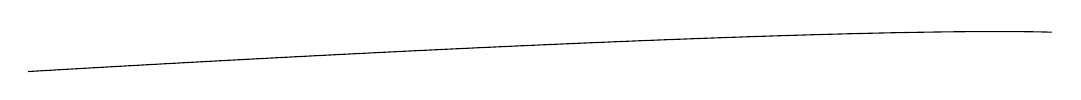
\begin{tikzpicture}\draw(0,0)..controls(6,.35)and(11,.55)..(13,.5);\end{tikzpicture}}

Cas important \(N=2m+1\), à \unsure{prouver} alors
\[
A^{m+1}(X)\equiv0\qquad(\text{et }A^i(X)\equiv0\text{ si }i\geq m+1)
\]
[Cas \(N=2m\), alors \(N^m(X)\equiv0\) i.e. \(J^m(X)\equiv A^m(X)\),

et \(A^{m+1}(X)\equiv0\ \unsure{\sim}\ (\text{et }A^{\deleted{m}\inserted{i}}(X)\equiv0\text{ si }i\geq m+1)\)]
\margin{108}
